\documentclass[12pt]{article}

% --------------------
% Packages
% --------------------
\usepackage[margin=1in]{geometry}
\usepackage{amsmath, amssymb, amsfonts}
\usepackage{mathtools}
\usepackage{enumitem}
\usepackage{titlesec}
\usepackage{fancyhdr}
\usepackage[dvipsnames]{xcolor}
\usepackage[colorlinks=true,linkcolor=blue]{hyperref}
\usepackage{physics}
\usepackage{tikz}
\usetikzlibrary{positioning}
\usetikzlibrary{calc,angles,quotes,spy}
\usepackage{cancel}
\usepackage{array}
\usepackage{tcolorbox}
\usepackage[useregional]{datetime2} % optional formatting
\usepackage[outline]{contour} % glow around text
\usetikzlibrary{patterns,snakes}
\usetikzlibrary{arrows.meta} % for arrow size

\colorlet{xcol}{blue!70!black}
\colorlet{darkblue}{blue!40!black}
\colorlet{myred}{red!65!black}
\tikzstyle{mydashed}=[xcol,dashed,line width=0.25,dash pattern=on 2.2pt off 2.2pt]
\tikzstyle{axis}=[->,thick] %line width=0.6
\tikzstyle{ell}=[{Latex[length=3.3,width=2.2]}-{Latex[length=3.3,width=2.2]},line width=0.3]
\tikzstyle{dx}=[-{Latex[length=3.3,width=2.2]},darkblue,line width=0.3]
\tikzstyle{ground}=[preaction={fill,top color=black!10,bottom color=black!5,shading angle=20},
                    fill,pattern=north east lines,draw=none,minimum width=0.3,minimum height=0.6]
\tikzstyle{mass}=[line width=0.6,red!30!black,fill=red!40!black!10,rounded corners=1,
                  top color=red!40!black!20,bottom color=red!40!black!10,shading angle=20]
\tikzstyle{spring}=[line width=0.8,blue!7!black!80,snake=coil,segment amplitude=5,segment length=5,line cap=round]
\tikzset{>=latex} % for LaTeX arrow head
\tikzstyle{force}=[->,myred,very thick,line cap=round]
\def\tick#1#2{\draw[thick] (#1)++(#2:0.1) --++ (#2-180:0.2)}

% --------------------
% Page Style
% --------------------
\pagestyle{fancy}
\fancyhf{}
\fancyhead[L]{Physics II}
\fancyhead[R]{Lecture Notes}
\fancyfoot[C]{\thepage}
% --------------------
% Section Formatting
% --------------------
\titleformat{\section}
  {\normalfont\Large\bfseries}{Lecture \thesection}{1em}{}

\titleformat{\subsection}
  {\normalfont\large\bfseries}{\thesubsection}{1em}{}

\setlist[itemize]{noitemsep}

% --------------------
% Custom Commands
% --------------------
\newcommand{\R}{\mathbb{R}}
\newcommand{\mat}[1]{\begin{pmatrix} #1 \end{pmatrix}}
\newcommand{\changelink}[2]{\hyperref[#1]{#2}}

% Compact style: DD/MM/YY + 12-hour time
\newcommand{\compactdatetime}{%
  % Date: DD/MM/YY
  \the\day/\the\month/\the\numexpr\year-2000\relax\ %
  % Time: 12-hour
}
% --------------------
% Document Info
% --------------------
\title{\vspace{-2em}Physics II — Lecture Notes}
\author{Based on class notes by Jake Bobowski}

% --------------------
% Document
% --------------------
\begin{document}

\maketitle
\vspace{-1em}
\noindent\text{Click on a section to jump there!}
\tableofcontents
\newpage

\begin{tcolorbox}[
  title={Recent Updates \hfill Last updated: 14/1/26 2:30PM},
  colback=gray!5,
  colframe=black!40,
  boxrule=0.5pt,
  arc=4pt,
  fonttitle=\bfseries
]
\begin{itemize}

  \item \textbf{Jan 14:} Added \changelink{sec:lecture4-coulombs-law}{Lecture 4 - Coulombs Law}
  \subitem  Added \changelink{sec:lecture4.1-vector-form}{Lecture 4 - The Vector Form of Coulombs Law}

  \item \textbf{Jan 12:} Added \changelink{sec:lecture3-electric-charge}{Lecture 3 - Electric Charge}  
  \subitem Added \changelink{sec:lecture3.1-charging-by-induction}{3.1 Charging by Induction} 

  \item \textbf{Jan 11}: Added onto:
  \subitem\changelink{sec:lecture2.4-pendulum-with-small-angle}{Subsection 2.4 -- Pendulum with the Small Angle Approximation}
  \subitem Fixed/added graphics, small math errors, and clarifications: 
  \subitem\changelink{sec:lecture2.1-mass-on-spring}{Subsection 2.1 -- Mass on a Spring}
  \subitem\changelink{sec:lecture2.2-pendulum}{Subsection 2.2 -- Pendulum}
  \subitem\changelink{sec:aside2.2.1-rotational-motion}{Aside -- Rotational Motion}
  \subitem\changelink{sec:aside2.3.1-small-angle-approx}{Aside -- Small Angle Approximation}
  
  \item \textbf{Jan 10}: Added illustration to \changelink{sec:lecture2-rotational-motion}{Lecture 2 -- Concepts of Rotational Motion and General Oscillations}
  \subitem Added illustration of atom (Subsection 1.1.1)
  \subitem Added illustration of $\vec{F}$ and $\vec{E}$ (Subsection 1.1.2)
  
  
  \item \textbf{Jan 9}: Added content to Lecture 2:
  \subitem\changelink{sec:lecture2-rotational-motion}{Lecture 2 -- Concepts of Rotational Motion and General Oscillations}
  \subitem\changelink{sec:lecture2.1-mass-on-spring}{Subsection 2.1 -- Mass on a Spring}
  \subitem\changelink{sec:lecture2.2-pendulum}{Subsection 2.2 -- Pendulum}
  \subitem\changelink{sec:aside2.2.1-rotational-motion}{Aside -- Rotational Motion}
  \subitem\changelink{sec:aside2.3.1-small-angle-approx}{Aside -- Small Angle Approximation}
\end{itemize}
\end{tcolorbox}

% =====================================================
\newpage

\section{Electricity and Magnetism Introduction}
\subsection{The Electrostatic Force}
The electrostatic force is one of the forces that we experience continuously.

\subsubsection{The Atom}
All physical objects are made out of atoms. It contains:
\begin{enumerate}
    \item A positive core, which is the \textbf{nucleus}, and
    \item surrounded by a cloud of electrons. 
\end{enumerate}
\begin{center}
    \begin{tikzpicture}[scale=1.5]

% --- Electron cloud (very irregular boundary) ---
\draw[thick, blue]
  plot[smooth cycle, tension=0.6]
  coordinates {
    (2.4,0.3)
    (1.9,1.6)
    (0.7,2.3)
    (-0.9,2.0)
    (-2.0,1.1)
    (-2.4,0.0)
    (-2.1,-1.2)
    (-1.2,-2.2)
    (0.4,-2.4)
    (1.6,-1.9)
    (2.3,-0.9)
  };

% --- Many negative charges in the cloud ---
\foreach \x/\y in {
  1.5/0.7, 0.8/1.5, -0.4/1.7, -1.3/1.0,
  -1.8/0.2, -1.2/-0.8, -0.3/-1.6, 0.7/-1.8,
  1.6/-1.0, 1.9/-0.1, 0.2/0.6, -0.6/0.3
}{
  \node[blue] at (\x,\y) {$-$};
}

% --- Nucleus (denser, multiple pluses) ---
\draw[thick] (0,0) circle (0.18);

\foreach \x/\y in {
  0/0, 0.05/0.05, -0.05/-0.05, 0.06/-0.04
}{
  \node at (\x,\y) {\small $+$};
}

% --- Nucleus label ---
\draw[->] (0.35,0.25) -- (1.0,0.7)
  node[right] {$r_n \sim 10^{-15}\,\mathrm{m}$};

% --- Atomic radius label ---
\draw[->, blue] (-1.7,1.8) -- (-2.5,2.4)
  node[left, blue] {$r_a \sim 10^{-11}\,\mathrm{m}$};

\end{tikzpicture}    
\end{center}

\vspace{1em}

\noindent For a typical atom like carbon, the nucleus' radius is around $3\times10^{-15}$m. On the other hand, the atom's radius is $\approx$ $7\times10^{-11}$m. The ratio of these two radii:
\begin{align*}
    \frac{r_{\text{atom}}}{r_{\text{nucleus}}} = \frac{10^{-11}}{10^{-15}} = 10^4
\end{align*}

\noindent Therefore, the atom is mostly "empty" space with the vast majority of its mass in a tiny core. To get a sense of this: 

\[
\begin{aligned}
\frac{d_{\text{moon}}}{r_{\text{earth}}} \approx 60
\end{aligned}
\qquad
\frac{d_{\text{Sun-Earth}}}{r_{\text{Sun}}} \approx 215
\]

\subsubsection{Electrostatic Repulsion}
When one touches a table, or any other object, one does not physically come in contact with anything. What on experiences is the electric repulsion between $e^-$ (electrons) in the atoms of one's hand and those of the table.

\vspace{0.5em}

\noindent Then how does one experience contact forces such as the normal force? Just as the gravitational force does not require contact and acts at a distance via a gravitational field, electric charges establish electric fields that can exert forces on other charges. 

\vspace{1.5em}

\noindent\textbf{Core Concept.} The electrostatic force is along the direction of the electric field, denoted by $\vec{E}$, which is a vector. 
\begin{center}
    \begin{tikzpicture}[scale=2.5]

% Charges
\node at (-1,-0.25) {$e^{-}$};
\node at (2,0.25) {$p^{+}$};

\fill (-1,0) circle (1.2pt);
\fill (2,0) circle (1.2pt);

% Separation
\draw[dashed] (-1,0) -- (1,0);

% Electric field at proton (longer)
\draw[->, thick, blue]
  (2,0) -- (0.8,0)
  node[midway, above] {$\vec{E}$};

% Force on proton (shorter)
\draw[->, thick, green!70!black]
  (2,0) -- (1.3,0)
  node[midway, below] {$\vec{F}$};

\end{tikzpicture}
\end{center}

\subsubsection{Magnets and Electricity}

\textbf{Core Concept.} The magnetic force is perpendicular to both:
\begin{enumerate}
    \item the direction of $\vec{B}$,
    \item and the direction of the charge's velocity, $\vec{v}$.
\end{enumerate}

\vspace{0.5em}

\begin{center}
    \begin{tikzpicture}[scale=2.5]
        \draw[->, thick] (0,0) -- (1.2,0)
    node[right] (v) {$\vec{v}$};

  % Into-the-page vector
  \node at (0,0) {$\otimes$};
  \node[above right=1pt] {$\vec{B}$};

  % Force vectors
  \draw[->, thick] (0,0) -- (0,1.2) node[above] {$\vec{F_{b}}$};
  \draw[->, thick] (0,0) -- (1.2,0) node[right] {$\vec{v}$};

\end{tikzpicture}
\end{center}

\noindent In this picture, we can conclude that $\vec{F_b} \perp \vec{B} \perp \vec{v}$. This is a special case of circular motion as $\vec{F_b} \perp \vec{v}$.


% =====================================================
\section{Concepts of Rotational Motion and General Oscillations}
\label{sec:lecture2-rotational-motion}

\subsection{Mass on a Spring}
\label{sec:lecture2.1-mass-on-spring}

\noindent Here is a mass on a spring in its \textbf{equilibrium position}.

\begin{center}
    % HORIZONTAL spring - axis, rest position
    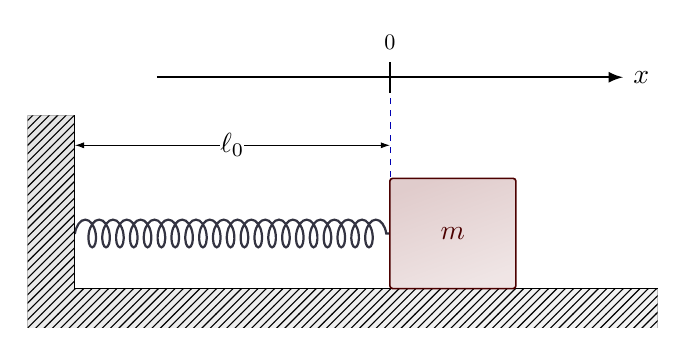
\begin{tikzpicture}[scale = 2]
  \def\H{1.1}  % wall height
  \def\T{0.3}  % wall thickness
  \def\W{3.7}  % ground length
  \def\D{0.25} % ground depth
  \def\h{0.7}  % mass height
  \def\w{0.8}  % mass width
  \def\x{2.0}  % mass x position
  \def\y{1.22*\H} % x axis y position
  
  % AXIS
  \draw[mydashed] (\x,0.9*\h) --++ (0,\y-0.9*\h);
  \draw[axis] (\x-0.4*\W,\y) -- (\x+0.4*\W,\y) node[right] {$x$};
  \tick{\x,\y}{-90} node[scale=0.8,above=0.05] {$0$};
  \draw[ell] (0,1.3*\h) --++ (\x,0) node[midway,fill=white,inner sep=0] {$\ell_0$};
  
  % SPRING & MASS
  \draw[spring] (0,\h/2) --++ (\x,0);
  \draw[ground] (0,0) |-++ (-\T,\H) |-++ (\T+\W,-\H-\D) -- (\W,0) -- cycle;
  \draw (0,\H) -- (0,0) -- (\W,0);
  \draw[mass] (\x,0) rectangle++ (\w,\h) node[midway] {$m$};
  
\end{tikzpicture}
\end{center}


\noindent Here is its \textbf{extended} position:

\begin{center}
    % HORIZONTAL spring - axis, extended
    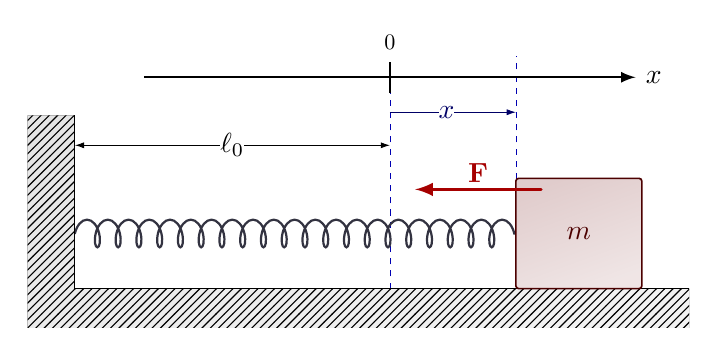
\begin{tikzpicture}[scale = 2]
  \def\H{1.1}  % wall height
  \def\T{0.3}  % wall thickness
  \def\W{3.9}  % ground length
  \def\D{0.25} % ground depth
  \def\h{0.7}  % mass height
  \def\w{0.8}  % mass width
  \def\x{2.0}  % mass x position
  \def\dx{0.8} % extension
  \def\y{1.22*\H} % x axis y position
  \def\F{0.8}  % force
  
  % AXIS
  \draw[mydashed] (\x,0) --++ (0,\y) (\x+\dx,0) --++ (0,1.1*\y);
  \draw[axis] (\x-0.4*\W,\y) -- (\x+0.4*\W,\y) node[right] {$x$};
  \tick{\x,\y}{-90} node[scale=0.8,above=0.05] {$0$};
  \draw[ell] (0,1.3*\h) --++ (\x,0) node[midway,fill=white,inner sep=0] {$\ell_0$};
  \draw[dx] (\x,1.6*\h) --++ (\dx,0) node[pos=0.45,fill=white,inner sep=0] {$x$};
  
  % SPRING & MASS
  \draw[spring,segment length=7.5] (0,\h/2) --++ (\x+\dx,0);
  \draw[ground] (0,0) |-++ (-\T,\H) |-++ (\T+\W,-\H-\D) -- (\W,0) -- cycle;
  \draw (0,\H) -- (0,0) -- (\W,0);
  \draw[mass] (\x+\dx,0) rectangle++ (\w,\h) node[midway] {$m$};
  \draw[force] (\x+\dx+0.2*\w,0.9*\h) --++ (-\F,0) node[midway,right=1,above=-0.05] {$\vb{F}$};
  
\end{tikzpicture}
\end{center}

\vspace{1em}

\noindent Here is its \textbf{compressed} position:

\begin{center}
    % HORIZONTAL spring - axis, compressed
    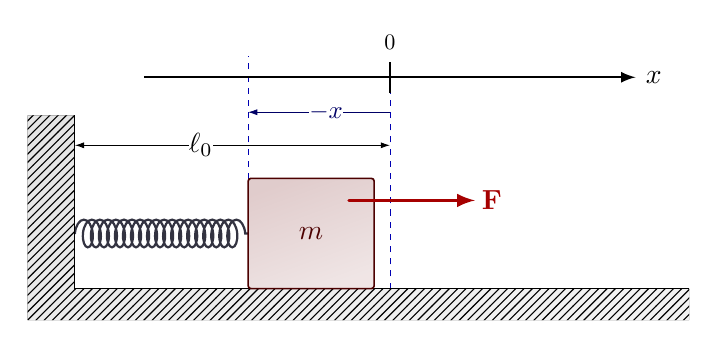
\begin{tikzpicture}[scale = 2]
  \def\H{1.1} % wall height
  \def\T{0.3} % wall thickness
  \def\W{3.9} % ground length
  \def\D{0.2} % ground depth
  \def\h{0.7} % mass height
  \def\w{0.8} % mass width
  \def\x{2.0} % mass x position
  \def\dx{0.9} % extension
  \def\y{1.22*\H} % x axis y position
  \def\F{0.8} % force
  
  % AXIS
  \draw[mydashed] (\x,0) --++ (0,\y) (\x-\dx,0) --++ (0,1.1*\y);
  \draw[axis] (\x-0.4*\W,\y) -- (\x+0.4*\W,\y) node[right] {$x$};
  \tick{\x,\y}{-90} node[scale=0.8,above=0.05] {$0$};
  \draw[ell] (0,1.3*\h) --++ (\x,0) node[pos=0.4,fill=white,inner sep=0] {$\ell_0$};
  \draw[dx] (\x,1.6*\h) --++ (-\dx,0)
    node[pos=0.45,fill=white,inner sep=0,scale=0.9] {$-x$};
  
  % SPRING & MASS
  \draw[spring,segment length=2.9] (0,\h/2) --++ (\x-\dx,0);
  \draw[ground] (0,0) |-++ (-\T,\H) |-++ (\T+\W,-\H-\D) -- (\W,0) -- cycle;
  \draw (0,\H) -- (0,0) -- (\W,0);
  \draw[mass] (\x-\dx,0) rectangle++ (\w,\h) node[midway] {$m$};
  \draw[force] (\x-\dx+0.8*\w,0.8*\h) --++ (\F,0) node[below=0,right=-0.05] {$\vb{F}$};
  
\end{tikzpicture}
\end{center}


\noindent The spring force on a mass $m$ is given through the formula $F_s = -kx$. This is classified as a restoring force.

\vspace{1em}

\noindent Newton's 2nd Law states that $F = ma$. Recall that:
\begin{align*}
    a = \dfrac{dv}{dt}\ = \dfrac{d}{dt}\left(\dfrac{dx}{dt}\right) = \dfrac{d^2x}{dt^2} \\
\end{align*}
\noindent And so substituting in for $a$: 

\begin{equation}
    m\dfrac{d^2x}{dt^2} = -kx
\end{equation}

\noindent To find $x(t)$, or the time evolution of $x$, we need a function that after taking two derivatives, returns the original function with a negative sign. Let us try the function $A\cos{(\omega t})$, where $A$ is the amplitude/initial displacement, and $\omega$ is the angular frequency. As a consequence of the chain rule: 

\begin{align*}
    \vec{v} = \dfrac{dx}{dt} = -\omega A\cos{(\omega t)} 
\end{align*}

Differentiating the second time:

\begin{equation}
   \vec{a} = \dfrac{d\vec{v}}{dt} = -\omega^{2} A\cos{(\omega t)}
\end{equation}

\begin{align*}
    \therefore \text{ We can say } A\cos{(\omega t) = x \Rightarrow \dfrac{d^2 x}{dt^2}= -\omega^{2} x}.
\end{align*}

Substituting (2) into (1):
\begin{align*}
    m(-\omega^{2}x)&=-kx \\
    m(\cancel{-}\omega^{2}\cancel{x})&=\cancel{-}k\cancel{x} \\
    \therefore w^2 = \frac{k}{m} \text{ or } w &= \sqrt{\frac{k}{m}}
\end{align*}

where $\sqrt{\frac{k}{m}}$ is the angular frequency of a mass on a spring.

\vspace{1em}

Recall that angular frequency, $\omega$, is $2\pi f$, where $f$ is the frequency or cycles/second. 
\begin{align*}
    \therefore \omega = 2 \pi f \\
    \text{ where } f= \frac{1}{T}.
\end{align*}

So, 
\begin{align*}
    T = 2\pi\sqrt{\frac{m}{k}}
\end{align*}

Notice $T$ of the motion is independent of the amplitude. 

% =====================================================

\subsection{Pendulum}
\label{sec:lecture2.2-pendulum}
Let us try to relate the problem of an oscillating pendulum to the mass on a spring. We can define a coordinate system wherein the $x$-axis (dashed line in blue) is a line tangent to the arc travelled by the bob, and the $y$-axis is along a string holding the bob in place.

\begin{center}
    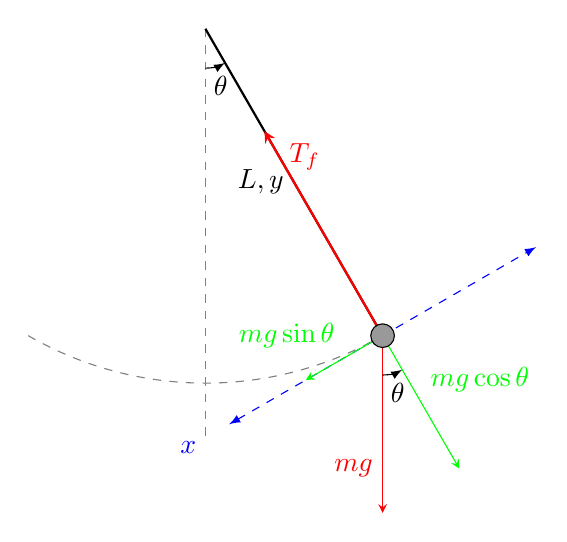
\begin{tikzpicture}[scale = 1.5]
    % save length of g-vector and theta to macros
    \pgfmathsetmacro{\Gvec}{1.5}
    \pgfmathsetmacro{\myAngle}{30}
    \pgfmathsetmacro{\pendulumLength}{3}
    
    % calculate lengths of vector components
    \pgfmathsetmacro{\Gcos}{\Gvec*cos(\myAngle)}
    \pgfmathsetmacro{\Gsin}{\Gvec*sin(\myAngle)}

    \coordinate (centro) at (0,0);
    \draw[dashed,gray,-] (centro) -- ++ (0,-3.5) node (mary) [black,below]{$ $};
    
    % 1. Dotted circular arc path
    \draw[dashed, gray] (270-\myAngle:\pendulumLength) arc (270-\myAngle:270+\myAngle:\pendulumLength);

    % Pendulum Arm (y-axis direction)
    \draw[thick] (centro) -- ++(270+\myAngle:\pendulumLength) coordinate (bob)
      node[midway, left] {$L,y$};
    
    % Top Angle
    \pic [draw, ->, "$\theta$", angle eccentricity=1.5] {angle = mary--centro--bob};

    % 2. Extended Tangent x-axis (Dotted)
    % This draws a line through the bob, perpendicular to the string
    \draw[dashed, blue, <->] ($(bob)!1.5cm!90:(centro)$) -- ($(bob)!1.5cm!-90:(centro)$);
    \node[blue] at ($(bob)!1.9cm!90:(centro)$) {$x$};

    % 3. Tension Force (T_f) - BLUE
    \draw [red,-stealth, thick] (bob) -- ($(bob)!2.0cm!(centro)$) 
      node[very near end, right] {$T_f$};

    % Gravity Components
    % Radial component pointing away from centro (mg cos theta)
    \draw [green, -stealth] (bob) -- ($(bob)!-\Gcos cm!(centro)$)
      coordinate (gcos)
      node[midway,above right] {$mg\cos\theta$};
      
    % Tangential component (mg sin theta)
    \draw [green, -stealth] (bob) -- ($(bob)!\Gsin cm!90:(centro)$)
      coordinate (gsin)
      node[midway,above left] {$mg\sin\theta$};
      
    % Gravity Vector
    \draw [red, -stealth] (bob) -- ++(0,-\Gvec)
      coordinate (g)
      node[near end,left] {$mg$};
      
    % Bottom Angle
    \pic [draw, ->, "$\theta$", angle eccentricity=1.5] {angle = g--bob--gcos};
    
    % The Bob
    \filldraw [fill=black!40,draw=black] (bob) circle[radius=0.1];
\end{tikzpicture}
\end{center}

\noindent We have decomposed our forces into components along the $x$ and $y$ axes. We will analyze the net force along the $x$ and $y$ directions. In the $y$-direction:
\begin{align*}
    F_y = ma_y = T_f -mg\cos\theta = 0
\end{align*}

We have no up and down motion so this is equal to 0,
\begin{align*}
    \therefore T_f = mg\cos\theta
\end{align*}

In the x-direction: 
\begin{align*}
    F_x = ma_x = mg\sin\theta \\
    F_x = \cancel{m}a_x = \cancel{m}g\sin\theta
\end{align*}
\begin{equation}
    \therefore a_x = -g\sin\theta
\end{equation}

\noindent Equation (3) is not quite the same as the mass on the spring. We can make some manipulations to make it similar. 

% =====================================================

\subsubsection{Aside: Rotational Motion}
\label{sec:aside2.2.1-rotational-motion}
\vspace{1em}

\[
\begin{tabular}{m{5cm} @{\hspace{1cm}} m{5cm}} % '@' adds specific spacing between columns
    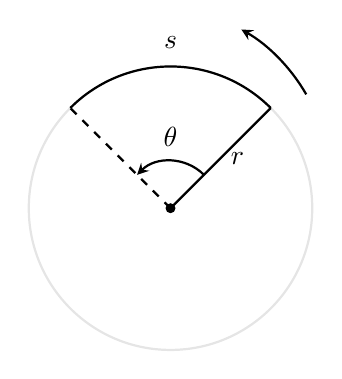
\begin{tikzpicture}[>=stealth, thick, scale=1.5]
        % 1. Draw the full circle in light gray
        \draw[gray!20] (0,0) circle (1.2cm);
        
        % 2. Draw the 90-degree "Pizza Slice" pointing up
        \coordinate (O) at (0,0);
        \draw (O) -- (45:1.2cm) node[midway, right] {$r$};
        \draw[dashed] (O) -- (135:1.2cm) node[midway, left]{};
        \draw[thick] (45:1.2cm) arc (45:135:1.2cm);
        
        % 3. Label for the arc 's'
        \node at (90:1.4cm) {$s$};
        
        % 4. Angle label theta inside
        \draw [->] (45:0.4cm) arc (45:135:0.4cm);
        \node at (90:0.6cm) {$\theta$};

        % 5. External rotation arrow
        \draw[->] (40:1.5cm) arc (30:60:1.5cm);
        
        % Origin point
        \fill (O) circle (1.2pt);
    \end{tikzpicture}
    & 
    % Wrap the table in a minipage aligned to the top [t]
    \begin{minipage}[t]{4cm}
        \vspace{-1cm} % Adjust this value to move the text up or down exactly where you want it
        \begin{tabular}{l}
            Circumference is $C = 2 \pi r$, \\
            the angle for a round trip on the \\
            circumference.
        \end{tabular}
    \end{minipage}
\end{tabular}
\]

\vspace{1em}

\[
\begin{tabular}{m{5cm} @{\hspace{1cm}} m{5cm}} % '@' adds specific spacing between columns
    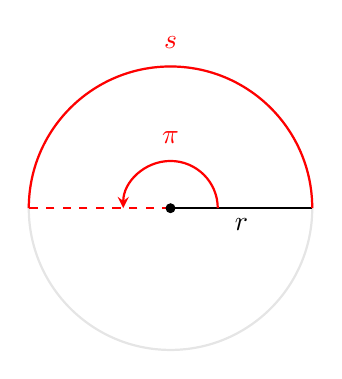
\begin{tikzpicture}[>=stealth, thick, scale=1.5]
    % 1. Draw the full circle in light gray
    \draw[gray!20] (0,0) circle (1.2cm);
    
    % 2. Define Center
    \coordinate (O) at (0,0);
    
    % 3. Draw the horizontal radius (Solid, to the right)
    % 0:1.2cm means 0 degrees (horizontal)
    \draw (O) -- (0:1.2cm) node[midway, below] {$r$};

    \node[red] at (90:1.4cm) {$s$};
    
    % 4. Draw the opposite radius (Dashed, to the left)
    % 180:1.2cm is the far left
    \draw[red, dashed] (O) -- (180:1.2cm);
    
    \draw[thick, red] (0:1.2cm) arc (0:180:1.2cm);

    % 5. Draw the angle arrow (theta = pi)
    % It starts at 0 degrees and sweeps to 180 degrees
    \draw [red, ->] (0.4,0) arc (0:180:0.4cm);
    \node[red] at (90:0.6cm) {$\pi$};

    % Origin point
    \fill (O) circle (1.2pt);
\end{tikzpicture}
    & 
    % Wrap the table in a minipage aligned to the top [t]
    \begin{minipage}[t]{4cm}
        \vspace{-1cm} % Adjust this value to move the text up or down exactly where you want it
        \begin{tabular}{l}
            Arclength is $S = \pi r$, \\
            the area travelled along our arc.
        \end{tabular}
    \end{minipage}
\end{tabular}
\]

\[
\begin{tabular}{m{5cm} @{\hspace{1cm}} m{5cm}}
    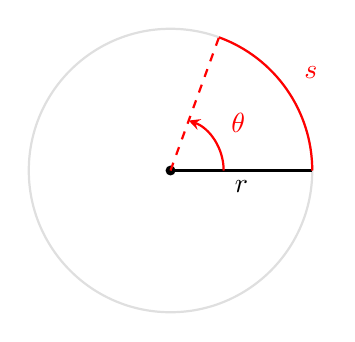
\begin{tikzpicture}[>=stealth, thick, scale=1.5]

        % Circle
        \draw[gray!25] (0,0) circle (1.2cm);

        % Center
        \coordinate (O) at (0,0);
        \fill (O) circle (1.2pt);

        % Radius lines
        \draw (O) -- (0:1.2cm) node[midway, below] {$r$};
        \draw[red, dashed] (O) -- (70:1.2cm);

        % Arc corresponding to angle theta
        \draw[thick, red] (0:1.2cm) arc (0:70:1.2cm);

        % Arc label s
        \node[red] at (35:1.45cm) {$s$};

        % Angle theta (radians)
        \draw[->, red] (0:0.45cm) arc (0:70:0.45cm);
        \node[red] at (35:0.7cm) {$\theta$};

    \end{tikzpicture}
    &
    \begin{minipage}[t]{4cm}
        \vspace{-1cm}
        \begin{tabular}{l}
            Arclength is $S = \theta r$, the \\
            angle traveled in radians.
        \end{tabular}
    \end{minipage}
\end{tabular}
\]




\vspace{0.5em}

% =====================================================


\subsection{Pendulum Continued}
What about the speed?
\begin{align*}
    \vec{v} = \dfrac{ds}{dt} = \dfrac{d}{dt}(r\theta)
\end{align*}

For circular motion, $r$ is constant so:
\begin{align*}
    \vec{v} = r\cdot\dfrac{d\theta}{dt}
\end{align*}

Finally, 
\begin{equation}
    a = \dfrac{d\vec{v}}{dt} = \dfrac{d}{dt} \left(r\dfrac{d\theta}{dt}\right) = r\dfrac{d^2 
    \theta}{dt^2}
\end{equation}

\vspace{1em}

Use Equation (4) in (3). For our pendulum, $r = L$.
\begin{align*}
    a_x = -g\sin\theta \\
    L\dfrac{d^2 
    \theta}{dt^2} = -g\sin\theta
\end{align*}

or

\begin{equation}
    \dfrac{d^2 \theta}{dt^2} = -\frac{g}{L}\sin\theta
\end{equation}

where $\theta$ is the angular position. Going back to our mass on a spring,
\begin{align*}
    \dfrac{d^2 x}{dt^2} = -\frac{k}{m}x
\end{align*}

\noindent where $x$ is the linear position of a mass on a spring. These are similar but not identical. We have $\sin\theta$ instead of $\theta$. We will consider the \textbf{small angle approximation.}

% =====================================================

\subsubsection{Aside: Small Angle Approximation}
\label{sec:aside2.3.1-small-angle-approx}


\begin{center}
    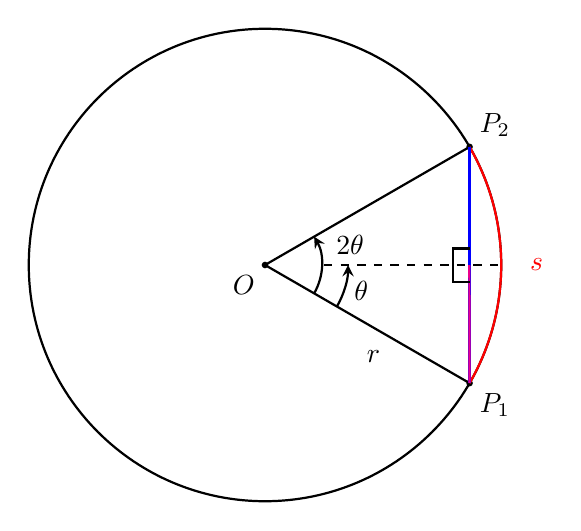
\begin{tikzpicture}[scale=3, thick]

% Circle
\draw (0,0) circle (1);

% Center and reference point
\coordinate (O) at (0,0);
\coordinate (A) at (1,0);
\coordinate (B) at (0.865,0);
\fill (O) circle (0.4pt) node[below left] {$O$};

% Points on circle
\coordinate (P1) at ({cos(-30)},{sin(-30)});
\coordinate (P2) at ({cos(30)},{sin(30)});

\fill (P1) circle (0.4pt) node[below right] {$P_1$};
\fill (P2) circle (0.4pt) node[above right] {$P_2$};

% Horizontal dashed reference line
\draw[dashed] (0.25,0) -- (1,0);

% Radii
\draw (O) -- (P1);
\draw (O) -- (P2);

% Radius label
\node at (-40:0.6) {$r$};

% Arc (s)
\draw[thick, red] (30:1) arc (30:-30:1);
\node[red] at (0:1.15) {$s$};

% Chord
\draw[blue] (P1) -- (P2);

\draw[magenta] (P1) -- (B);

% Foot of perpendicular (EXACT)
\coordinate (F) at ({cos(30)},0);

% Right angle marker (visible)
\pic [draw, angle radius=6pt] {right angle = P2--F--O};
\pic [draw, angle radius=6pt] {right angle = P1--F--O};

% Angle arcs
\pic [draw, -stealth, "$2\theta$", angle radius=20.5, angle eccentricity=1.5, above]
    {angle = P1--O--P2};

\pic [draw, -stealth, "$\theta$", angle radius=30, angle eccentricity=1.2]
    {angle = P1--O--A};

\end{tikzpicture}
\end{center}

\vspace{1em}
\noindent The distance from $P_1$ to $O$ (in magenta), is mathematically expressed as: 
\begin{align*}
    d = r\sin\theta
\end{align*}

\noindent And so it follows that the distance from $P_1$ to $P_2$ (in blue), which we will denote by distance $d$:
\begin{align*}
    d = 2r\sin\theta
\end{align*}

\vspace{1.5em}

\noindent The arc length (in red) between $P_1$ and $P_2$ has the length of
\begin{align*}
    s = 2r\theta
\end{align*}
by the definition of the radian measure.

\vspace{1.5em}
\noindent Comparing $s$ and $d$, it's clear that $s>d$:
\begin{align*}
    s = 2r\theta > 2r\sin\theta \\
    s = \cancel{2r}\theta > \cancel{2r}\sin\theta \\
\end{align*}

\noindent So,
\begin{align*}
     \therefore \theta > \sin\theta
\end{align*}

\vspace{1em}

\noindent If we consider a small angular displacement $2\theta$ between points $Q_1$ and $Q_2$, then the red arc and blue line are approximately the same length.

\begin{center}
    \input{figures/small-angle-approx2.tikz}
\end{center}

\noindent Here is a zoomed in view:


\begin{center}
    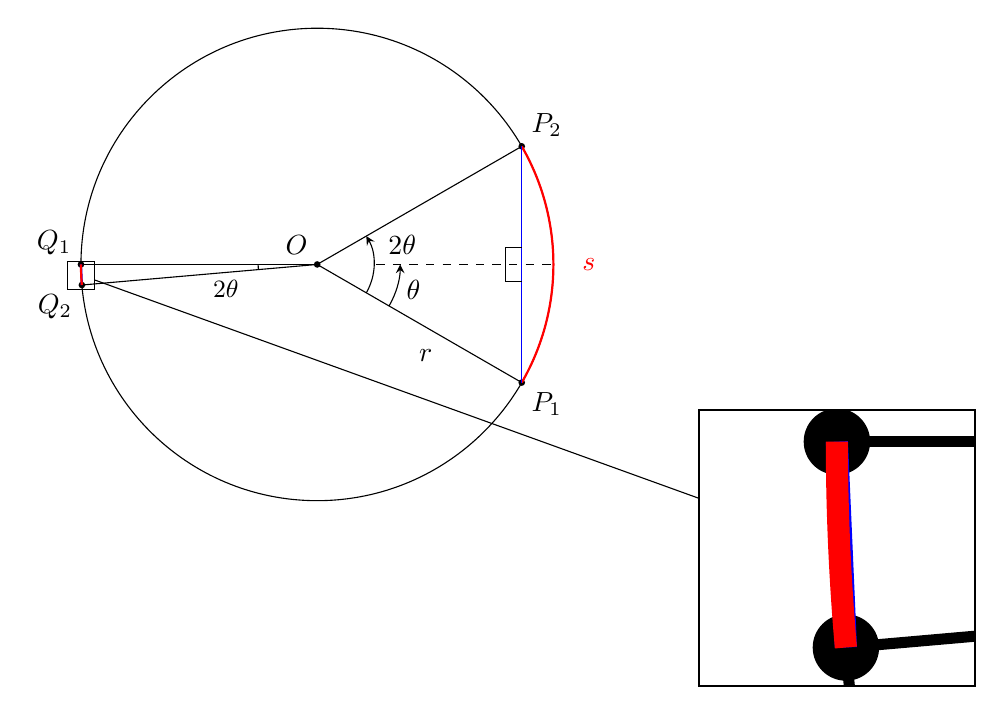
\begin{tikzpicture}[scale=3, thick,
    spy using outlines={
    rectangle,
    magnification=10,
    size=3.5cm,
    draw,
    thick,
    connect spies
  }]

% Circle
\draw (0,0) circle (1);

% Center and reference point
\coordinate (O) at (0,0);
\coordinate (A) at (1,0);
\fill (O) circle (0.4pt) node[above left] {$O$};

% Points on circle
\coordinate (P1) at ({cos(-30)},{sin(-30)});
\coordinate (P2) at ({cos(30)},{sin(30)});

\fill (P1) circle (0.4pt) node[below right] {$P_1$};
\fill (P2) circle (0.4pt) node[above right] {$P_2$};

% Horizontal dashed reference line
\draw[dashed] (0.25,0) -- (1,0);

% Radii
\draw (O) -- (P1);
\draw (O) -- (P2);

% Radius label
\node at (-40:0.6) {$r$};

% Arc (s)
\draw[thick, red] (30:1) arc (30:-30:1);
\node[red] at (0:1.15) {$s$};

% Chord
\draw[blue] (P1) -- (P2);

% Foot of perpendicular (EXACT)
\coordinate (F) at ({cos(30)},0);

% Right angle marker (visible)
\pic [draw, angle radius=6pt] {right angle = P2--F--O};
\pic [draw, angle radius=6pt] {right angle = P1--F--O};

% Angle arcs
\pic [draw, -stealth, "$2\theta$", angle radius=20.5, angle eccentricity=1.5, above]
    {angle = P1--O--P2};

\pic [draw, -stealth, "$\theta$", angle radius=30, angle eccentricity=1.2]
    {angle = P1--O--A};


% Small-angle wedge on left side
\coordinate (Q1) at (180:1);
\coordinate (Q2) at (185:1);

\spy on (-3,-0.135) in node at (2.2,-1.2);

\fill (Q1) circle (0.4pt) node[above left] {$Q_1$};
\fill (Q2) circle (0.4pt) node[below left] {$Q_2$};

\draw (O) -- (Q1);
\draw (O) -- (Q2);

% Small angle arc (2θ small)
\draw (180:0.25) arc (180:185:0.25);
\node at (195:0.40) {\small $2\theta$};

% Small straight-line distance (chord)
\draw[blue, thick] (Q1) -- (Q2);
% Small arc length
\draw[red, thick] (180:1) arc (180:185:1);
\end{tikzpicture}
\end{center}


\noindent Even closer:


\begin{center}
    \input{figures/small-angle-approx-zoom2.tikz}
\end{center}


With this, if $s \approx d$, then:
\begin{align*}
        2r\theta \approx 2r\sin\theta \\
        \cancel{2r}\theta \approx \cancel{2r}\sin\theta \\
\end{align*}

Therefore:

\begin{align*}
    \theta \approx \sin\theta
\end{align*}
when $\theta$ is small-angle approximation.

\subsection{Pendulum with the Small Angle Approximation}
\label{sec:lecture2.4-pendulum-with-small-angle}
\noindent In this case, equation (5) becomes:
\begin{align*}
    \dfrac{d^2\theta}{dt^2} \approx -\frac{g}{L}\theta
\end{align*}

\noindent which is mathematically identical to a mass on a spring:
\begin{align*}
    \dfrac{d^2x}{dt^2} = -\frac{k}{m}x
\end{align*}


\noindent So the solution for the angular position of the pendulum is:
\begin{align*}
    \theta = A\cos(\omega t) \text{ where } \omega = \sqrt{\frac{g}{L}}
\end{align*}

We also know that:
\begin{align*}
    \omega = \frac{2\pi}{T} \Rightarrow T = 2\pi\sqrt{\frac{L}{g}}
\end{align*}

\noindent These are the results of the pendulum when the amplitude of oscillation are small.

\noindent Note that the period $T$ is independent of the bob's mass and the amplitude of the oscillations.

\section{Electric Charge}
\label{sec:lecture3-electric-charge}
Imagine the following experiment:

\begin{itemize}
    \item Take two pieces of cellophane tape stuck to one another (i.e. sticky side to non-sticky side)
    \item Pull the pieces apart and isolate one another
    \item Repeat with the same two pieces of tape
    \item Take a fifth piece of tape that has not had any treatment (controlled)
\end{itemize}

\vspace{0.5em}
\begin{center}
    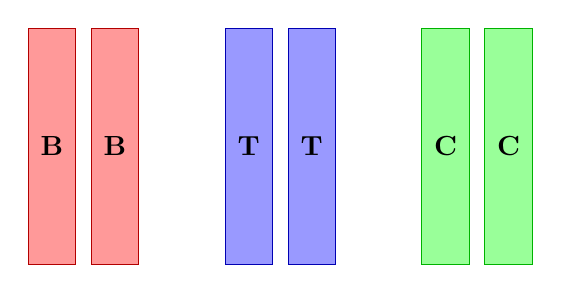
\begin{tikzpicture}

    % Define colors and labels in a list: {x-position/color/label}
    \foreach \x/\col/\txt in {
        0/red/B, 0.8/red/B,     % First pair
        2.5/blue/T, 3.3/blue/T, % Second pair
        5.0/green/C, 5.8/green/C % Third pair
    } {
        % Draw the "cellophane" box
        % fill opacity creates the translucent effect
        \draw[fill=\col, fill opacity=0.4, draw=\col!70!black] 
            (\x, 0) rectangle (\x+0.6, 3);
        
        % Label in the center of the box
        \node at (\x+0.3, 1.5) {\textbf{\txt}};
    }

\end{tikzpicture}
\end{center}

\noindent \textbf{Some observations:} 
\begin{itemize}
    \item The B pieces strongly repel one another, 
    \item The T pieces also strongly repel one another, 
    \item The T and B pieces attract, 
    \item and the C tape weakly attracts both T and B pieces!
\end{itemize}

\noindent When T and B tapes are pulled apart, some $e^{-}$ from one piece of tape are transferred to the other. The one that lost electrons became positively charged (defecit of $e^{-}$) and the one that gained electrons became negative. We can imply from our observations that:
\begin{enumerate}
    \item Like charges repel,
    \item opposites attract, 
    \item "control" has neither gained/lost electrons, therefore it is neutral, attracted to both + and -,
    \item and no electircal interaction between two neutral objects.
\end{enumerate}

\noindent To understand the 3rd observation, consider bringing a charged object next to a neutral one:

\begin{center}
    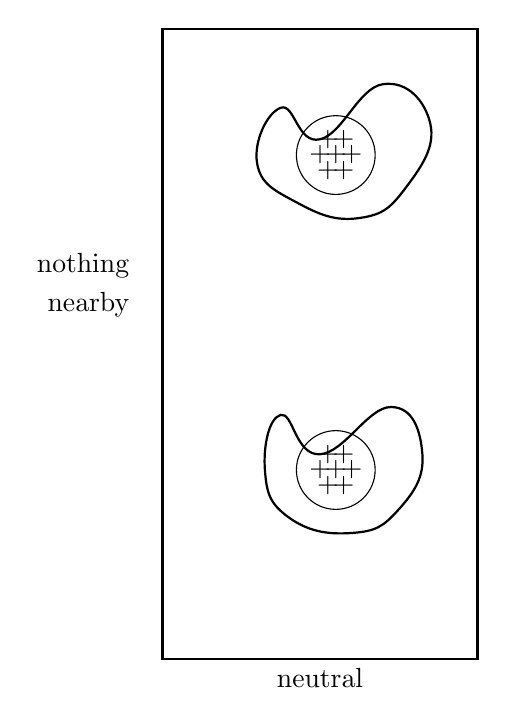
\begin{tikzpicture}[scale=1]

% Outer box
\draw[line width=1pt] (0,0) rectangle (4,8);

% ---------- Top atom ----------
% Electron cloud
\draw[line width=0.8pt]
  plot[smooth cycle, tension=0.8]
  coordinates {(2,6.6) (2.8,7.3) (3.4,6.8) (3.1,6.0)
               (2.5,5.6) (1.7,5.8) (1.2,6.3) (1.5,7.0)};

% Nucleus
\draw (2.2,6.4) circle (0.5);

% Many positive charges
\foreach \x/\y in {
  2.1/6.6, 2.3/6.6, 2.0/6.4, 2.2/6.4, 2.4/6.4,
  2.1/6.2, 2.3/6.2
}{
  \node at (\x,\y) {$+$};
}

% ---------- Bottom atom ----------
\draw[line width=0.8pt]
  plot[smooth cycle, tension=0.8]
  coordinates {(2,2.6) (2.9,3.2) (3.3,2.6) (3.0,1.9)
               (2.4,1.6) (1.6,1.8) (1.3,2.4) (1.5,3.1)};

\draw (2.2,2.4) circle (0.5);

\foreach \x/\y in {
  2.1/2.6, 2.3/2.6, 2.0/2.4, 2.2/2.4, 2.4/2.4,
  2.1/2.2, 2.3/2.2
}{
  \node at (\x,\y) {$+$};
}

% ---------- Labels ----------
\node[left] at (-0.3,5) {nothing};
\node[left] at (-0.3,4.5) {nearby};

\node[below] at (2,0) {neutral};

\end{tikzpicture}

\end{center}

\noindent Bringing a charged object:

\begin{center}
    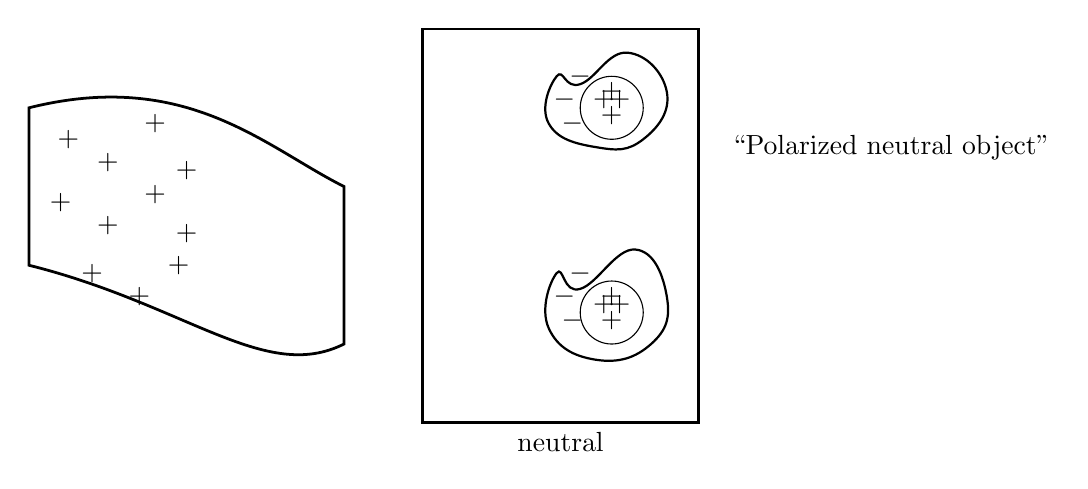
\begin{tikzpicture}[scale=1]

% ---------------- Charged rod ----------------
\draw[line width=1pt]
  (-4,5) .. controls (-2,5.5) and (-1,4.5) .. (0,4)
  -- (0,2)
  .. controls (-1,1.5) and (-2,2.5) .. (-4,3)
  -- cycle;

% Plus charges in rod
\foreach \x/\y in {
  -3.5/4.6, -3.0/4.3, -2.4/4.8, -2.0/4.2,
  -3.6/3.8, -3.0/3.5, -2.4/3.9, -2.0/3.4,
  -3.2/2.9, -2.6/2.6, -2.1/3.0
}{
  \node at (\x,\y) {$+$};
}

% ---------------- Neutral object box ----------------
\draw[line width=1pt] (1,1) rectangle (4.5,6);

% ---------- Top atom (polarized) ----------
\draw[line width=0.8pt]
  plot[smooth cycle, tension=0.8]
  coordinates {(3,5.3) (3.6,5.7) (4.1,5.2) (3.8,4.6)
               (3.2,4.5) (2.6,4.8) (2.7,5.4)};

% Nucleus shifted right
\draw (3.4,5.0) circle (0.4);

\foreach \x/\y in {
  3.3/5.1, 3.5/5.1, 3.4/4.9, 3.4/5.2
}{
  \node at (\x,\y) {$+$};
}

% Negative charges left
\foreach \x/\y in {
  2.8/5.1, 2.9/4.8, 3.0/5.4
}{
  \node at (\x,\y) {$-$};
}

% ---------- Bottom atom (polarized) ----------
\draw[line width=0.8pt]
  plot[smooth cycle, tension=0.8]
  coordinates {(3,2.7) (3.7,3.2) (4.1,2.6) (3.9,2.0)
               (3.2,1.8) (2.6,2.2) (2.7,2.9)};

\draw (3.4,2.4) circle (0.4);

\foreach \x/\y in {
  3.3/2.5, 3.5/2.5, 3.4/2.3, 3.4/2.6
}{
  \node at (\x,\y) {$+$};
}

\foreach \x/\y in {
  2.8/2.6, 2.9/2.3, 3.0/2.9
}{
  \node at (\x,\y) {$-$};
}

% ---------------- Labels ----------------
\node[right] at (4.8,4.5) {``Polarized neutral object''};
\node[below] at (2.75,1) {neutral};

\end{tikzpicture}

\end{center}

\begin{center}
    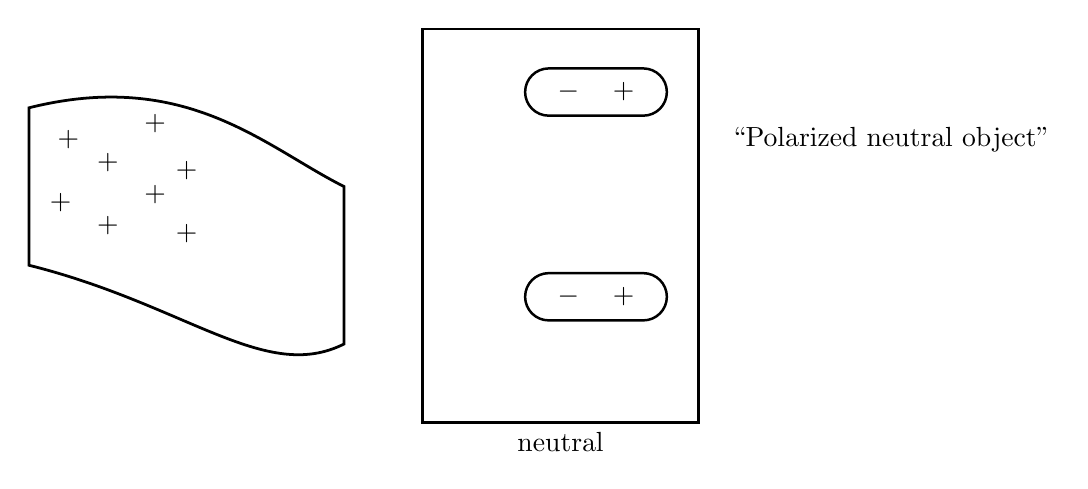
\begin{tikzpicture}[scale=1]

% ---------------- Charged rod ----------------
\draw[line width=1pt]
  (-4,5) .. controls (-2,5.5) and (-1,4.5) .. (0,4)
  -- (0,2)
  .. controls (-1,1.5) and (-2,2.5) .. (-4,3)
  -- cycle;

\foreach \x/\y in {
  -3.5/4.6, -3.0/4.3, -2.4/4.8, -2.0/4.2,
  -3.6/3.8, -3.0/3.5, -2.4/3.9, -2.0/3.4
}{
  \node at (\x,\y) {$+$};
}

% ---------------- Neutral object box ----------------
\draw[line width=1pt] (1,1) rectangle (4.5,6);

% ---------- Pill function ----------
% center (x,y), length L, radius r
\def\pill#1#2#3#4{
  \draw[line width=0.9pt]
    (#1-#3/2,#2-#4) --
    (#1+#3/2,#2-#4)
    arc[start angle=-90,end angle=90,radius=#4] --
    (#1-#3/2,#2+#4)
    arc[start angle=90,end angle=270,radius=#4] -- cycle;
}

% ---------- Top pill ----------
\pill{3.2}{5.2}{1.2}{0.3}
\node at (2.85,5.2) {$-$};
\node at (3.55,5.2) {$+$};

% ---------- Bottom pill ----------
\pill{3.2}{2.6}{1.2}{0.3}
\node at (2.85,2.6) {$-$};
\node at (3.55,2.6) {$+$};

% ---------------- Labels ----------------
\node[right] at (4.8,4.6) {``Polarized neutral object''};
\node[below] at (2.75,1) {neutral};

\end{tikzpicture}
\end{center}

\noindent The negative left edge is more strongly attarcted to the positibe rod than the positive right edge which is repelled by the rod. The force of attraction/repulsion depends on the distance between charges.

\subsection{Charging by Induction}
\label{sec:lecture3.1-charging-by-induction}
\noindent\textbf{Important Question:} Can we charge an object without touching it? Yes we can!

\vspace{1em}

\noindent In conductors, some electrons are free to move around the material. They are not tied to one particular atom. Consider the following:

\vspace{1em}

\noindent\textbf{Step A:} Place two neutral conductors in contact.

\begin{center}
    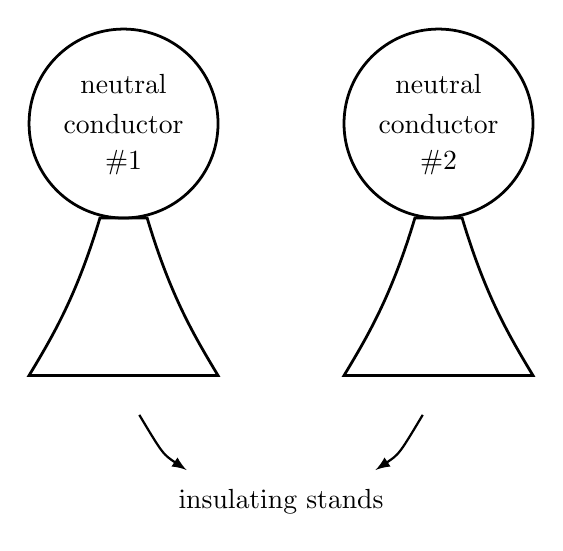
\begin{tikzpicture}[scale=1]

% ---------- Conductor 1 ----------
\draw[line width=1pt] (-2,4) circle (1.2);
\node at (-2,4.5) {neutral};
\node at (-2,4.0) {conductor};
\node at (-2,3.5) {\#1};

% Stand 1
\draw[line width=1pt]
  (-2.3,2.8) .. controls (-2.6,1.8) and (-2.9,1.3) .. (-3.2,0.8)
  -- (-0.8,0.8)
  .. controls (-1.1,1.3) and (-1.4,1.8) .. (-1.7,2.8)
  -- cycle;

% ---------- Conductor 2 ----------
\draw[line width=1pt] (2,4) circle (1.2);
\node at (2,4.5) {neutral};
\node at (2,4.0) {conductor};
\node at (2,3.5) {\#2};

% Stand 2
\draw[line width=1pt]
  (1.7,2.8) .. controls (1.4,1.8) and (1.1,1.3) .. (0.8,0.8)
  -- (3.2,0.8)
  .. controls (2.9,1.3) and (2.6,1.8) .. (2.3,2.8)
  -- cycle;

% ---------- Arrows & label ----------
\draw[->, line width=0.8pt] (-1.8,0.3) .. controls (-1.5,-0.2) .. (-1.2,-0.4);
\draw[->, line width=0.8pt] (1.8,0.3) .. controls (1.5,-0.2) .. (1.2,-0.4);

\node at (0,-0.8) {insulating stands};

\end{tikzpicture}
\end{center}

\noindent\textbf{Step B:} Bring a charged rod nearby (next to, not touching one of the conductors)

\begin{center}
    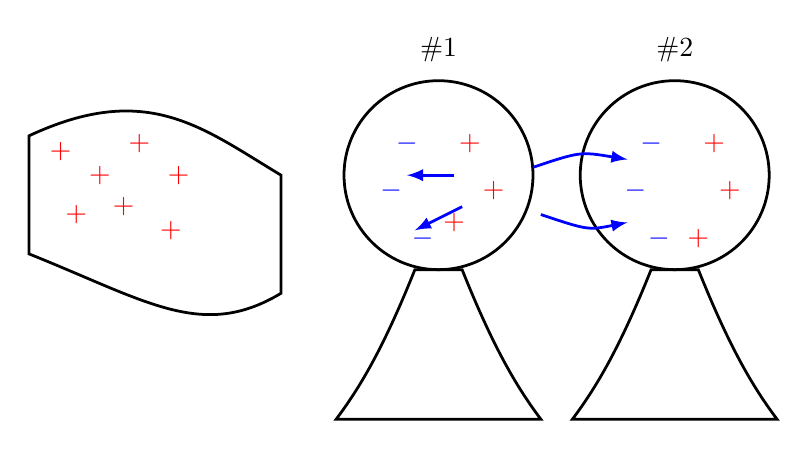
\begin{tikzpicture}[scale=1]

% ================= Charged rod =================
\draw[line width=1pt]
  (-6,4.5) .. controls (-4.5,5.2) and (-3.8,4.6) .. (-2.8,4)
  -- (-2.8,2.5)
  .. controls (-3.8,1.9) and (-4.5,2.4) .. (-6,3)
  -- cycle;

\foreach \x/\y in {
  -5.6/4.3, -5.1/4.0, -4.6/4.4, -4.1/4.0,
  -5.4/3.5, -4.8/3.6, -4.2/3.3
}{
  \node[red] at (\x,\y) {$+$};
}

% ================= Conductor 1 =================
\draw[line width=1pt] (-0.8,4) circle (1.2);
\node at (-0.8,5.6) {\#1};

% Fixed positive charges
\foreach \x/\y in {
  -0.4/4.4, -0.1/3.8, -0.6/3.4
}{
  \node[red] at (\x,\y) {$+$};
}

% Mobile electrons
\foreach \x/\y in {
  -1.2/4.4, -1.4/3.8, -1.0/3.2
}{
  \node[blue] at (\x,\y) {$-$};
}

\draw[->, blue, line width=1pt] (-0.6,4.0) -- (-1.2,4.0);
\draw[->, blue, line width=1pt] (-0.5,3.6) -- (-1.1,3.3);

% Stand 1
\draw[line width=1pt]
  (-1.1,2.8) .. controls (-1.5,1.8) and (-1.8,1.3) .. (-2.1,0.9)
  -- (0.5,0.9)
  .. controls (0.2,1.3) and (-0.1,1.8) .. (-0.5,2.8)
  -- cycle;

% ================= Conductor 2 =================
\draw[line width=1pt] (2.2,4) circle (1.2);
\node at (2.2,5.6) {\#2};

\foreach \x/\y in {
  2.7/4.4, 2.9/3.8, 2.5/3.2
}{
  \node[red] at (\x,\y) {$+$};
}

\foreach \x/\y in {
  1.9/4.4, 1.7/3.8, 2.0/3.2
}{
  \node[blue] at (\x,\y) {$-$};
}

\draw[->, blue, line width=1pt]
  (0.4,4.1) .. controls (1.0,4.3) .. (1.6,4.2);
\draw[->, blue, line width=1pt]
  (0.5,3.5) .. controls (1.1,3.3) .. (1.6,3.4);

% Stand 2
\draw[line width=1pt]
  (1.9,2.8) .. controls (1.5,1.8) and (1.2,1.3) .. (0.9,0.9)
  -- (3.5,0.9)
  .. controls (3.2,1.3) and (2.9,1.8) .. (2.5,2.8)
  -- cycle;
\end{tikzpicture}

\end{center}

\noindent\textbf{Step C:} With positive rod still in place, separate the conductors:

\begin{center}
    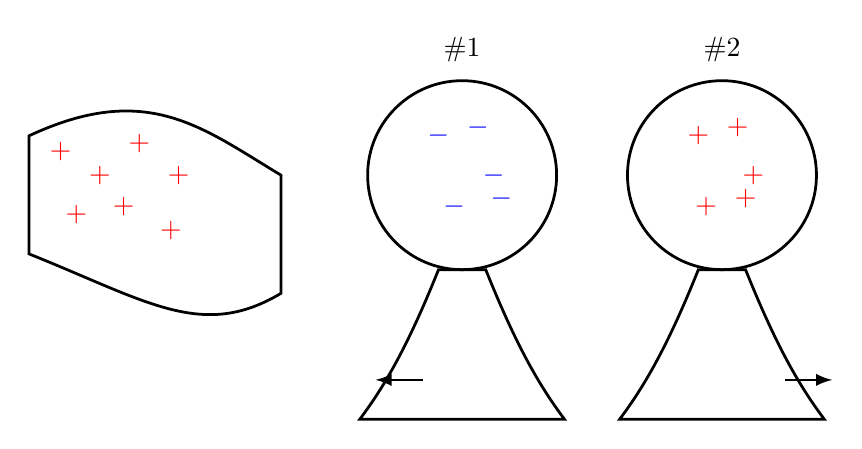
\begin{tikzpicture}[scale=1]

% ================= Charged rod =================
\draw[line width=1pt]
  (-6,4.5) .. controls (-4.5,5.2) and (-3.8,4.6) .. (-2.8,4)
  -- (-2.8,2.5)
  .. controls (-3.8,1.9) and (-4.5,2.4) .. (-6,3)
  -- cycle;

\foreach \x/\y in {
  -5.6/4.3, -5.1/4.0, -4.6/4.4, -4.1/4.0,
  -5.4/3.5, -4.8/3.6, -4.2/3.3
}{
  \node[red] at (\x,\y) {$+$};
}

% ================= Conductor #1 (negative) =================
\draw[line width=1pt] (-0.5,4) circle (1.2);
\node at (-0.5,5.6) {\#1};

\foreach \x/\y in {
  -0.8/4.5, -0.3/4.6, -0.1/4.0,
  -0.6/3.6,  0.0/3.7
}{
  \node[blue] at (\x,\y) {$-$};
}

% Stand 1
\draw[line width=1pt]
  (-0.8,2.8) .. controls (-1.2,1.8) and (-1.5,1.3) .. (-1.8,0.9)
  -- (0.8,0.9)
  .. controls (0.5,1.3) and (0.2,1.8) .. (-0.2,2.8)
  -- cycle;

% Separation arrow
\draw[->, line width=1pt] (-1.0,1.4) -- (-1.6,1.4);

% ================= Conductor #2 (positive) =================
\draw[line width=1pt] (2.8,4) circle (1.2);
\node at (2.8,5.6) {\#2};

\foreach \x/\y in {
  2.5/4.5, 3.0/4.6, 3.2/4.0,
  2.6/3.6, 3.1/3.7
}{
  \node[red] at (\x,\y) {$+$};
}

% Stand 2
\draw[line width=1pt]
  (2.5,2.8) .. controls (2.1,1.8) and (1.8,1.3) .. (1.5,0.9)
  -- (4.1,0.9)
  .. controls (3.8,1.3) and (3.5,1.8) .. (3.1,2.8)
  -- cycle;

% Separation arrow
\draw[->, line width=1pt] (3.6,1.4) -- (4.2,1.4);

\end{tikzpicture}

\end{center}

\noindent\textbf{Step D:} Remove charged rod. What remains is: 
\begin{itemize}
    \item One conductor with charge $-Q$,
    \item and one with charge $+Q$.
\end{itemize}


\section{Coulomb's Law}
\label{sec:lecture4-coulombs-law}
\noindent This law governs the forces between a pair of point charges. Take this illustration for instance.

\vspace{1em}

\begin{center}
    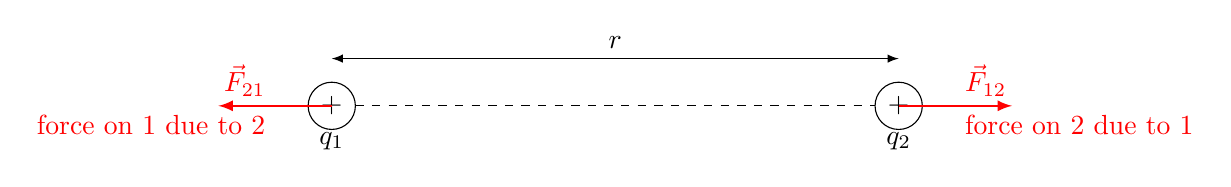
\begin{tikzpicture}[scale=1.2]

% Charges
\draw (0,0) circle (0.25);
\node at (0,0) {$+$};
\node[below=6pt] at (0,0) {$q_1$};

\draw (6,0) circle (0.25);
\node at (6,0) {$+$};
\node[below=6pt] at (6,0) {$q_2$};

% Separation line (dashed)
\draw[dashed] (0.25,0) -- (5.75,0);

% Distance r
\draw[<->] (0,0.5) -- (6,0.5);
\node[above] at (3,0.5) {$r$};

% Force on q1 due to q2
\draw[red,->,thick] (0,0) -- (-1.2,0);
\node[red,above left] at (-0.6,0) {$\vec F_{21}$};
\node[red,below left] at (-0.6,0) {force on 1 due to 2};

% Force on q2 due to q1
\draw[red,->,thick] (6,0) -- (7.2,0);
\node[red,above right] at (6.6,0) {$\vec F_{12}$};
\node[red,below right] at (6.6,0) {force on 2 due to 1};

\end{tikzpicture}

\end{center}

\noindent Remember that by Newton's third law: $\displaystyle|\vec{F}_{12}| = |\vec{F}_{21}|$. By careful experiments, we can deduce the following about the electric force between point charges. 

\vspace{0.5em}
\begin{enumerate}
    \item Force is directed along the line joining the two charges. 
    \item Force is attractive for opposite charges, repulsive for like charges. 
    \item Force is proportional to the inverse square of the separation distance, $r$:
    $\displaystyle |\vec{F}_{12}| = |\vec{F}_{21}| \propto \frac{1}{r^2}$
    \item Magnitude of the electric force is proportional to both $q_1$ and $q_2$: 
    $\displaystyle |\vec{F}_{12}| = |\vec{F}_{21}| \propto |q_1||q_2|$
\end{enumerate}

\noindent The magnitude of the electrostatic force is given by: 

\begin{align*}
    F = \frac{k_e q_1 q_2}{r^2}
\end{align*}

where $\displaystyle k_e \approx 8.99\times10^{9}\frac{Nm^2}{C^2}$.

\vspace{1em}

\noindent It is important to note that this is not derived from anything more fundamental, and based from experimental observations. We often see Coulomb's constant expressed as: 
\begin{align*}
    k_e = \frac{1}{4\pi\epsilon_{0}}
\end{align*}
where $\displaystyle \epsilon_{0}$ is the "permitivity of free space", and assigned the value of: 
\begin{align*}
    \epsilon_{0} \approx 8.85\times10^{-12}\frac{C^2}{Nm^2}
\end{align*}

\vspace{1em}

\begin{tcolorbox}[
  colback=yellow!10,
  colframe=yellow!60!black,
  title=\textbf{Example Question},
  fonttitle=\bfseries,
  boxrule=0.8pt,
  arc=2mm
]
Suppose we suspend identical masses $m$, each carrying an identical charge $q$, 
from strings of length $L$. Determine an expression for the equilibrium angle 
$\theta$. Below is a picture of the system:

\vspace{1em}

\begin{center}
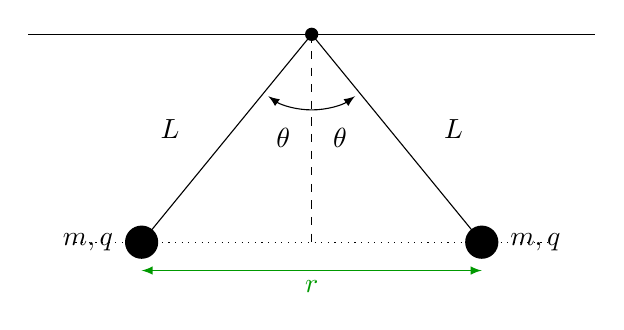
\begin{tikzpicture}[scale=1.2]

% Ceiling
\draw (-3,3) -- (3,3);

% Pivot
\fill (0,3) circle (2pt);

% Vertical symmetry line
\draw[dashed] (0,3) -- (0,0.75);

% Strings
\draw (0,3) -- (-1.8,0.8);
\draw (0,3) -- (1.8,0.8);

% Length labels
\node at (-1.5,2) {$L$};
\node at (1.5,2) {$L$};

% Angle labels
\draw[->] (0,2.2) arc[start angle=270,end angle=235,radius=0.8];
\node at (-0.3,1.9) {$\theta$};

\draw[->] (0,2.2) arc[start angle=270,end angle=305,radius=0.8];
\node at (0.3,1.9) {$\theta$};

% Masses
\fill (-1.8,0.8) circle (5pt);
\node[left] at (-2,0.8) {$m,q$};

\fill (1.8,0.8) circle (5pt);
\node[right] at (2,0.8) {$m,q$};

% Horizontal reference line
\draw[dotted] (-2.5,0.8) -- (2.5,0.8);

% Distance r
\draw[<->, green!60!black] (-1.8,0.5) -- (1.8,0.5);
\node[below, green!60!black] at (0,0.5) {$r$};

\end{tikzpicture}

\end{center}

\end{tcolorbox}

\begin{tcolorbox}[
  colback=white,
  colframe=green!50!black,
  boxrule=0.8pt,
  arc=1.5mm,
  title=\textbf{Solution},
  fonttitle=\bfseries
]
We should start by creating a diagram, here is the diagram with all the forces decomposed:

\begin{center}
    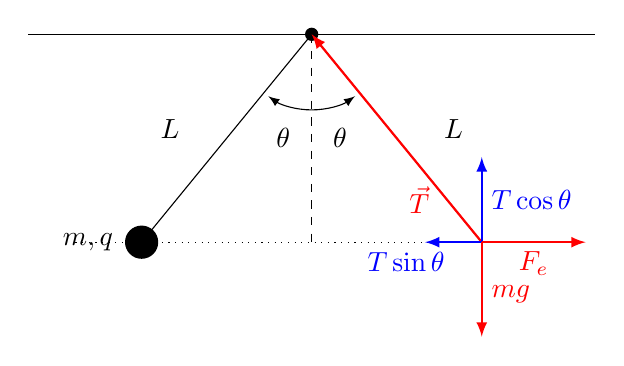
\begin{tikzpicture}[scale=1.2]

% Ceiling
\draw (-3,3) -- (3,3);

% Pivot
\fill (0,3) circle (2pt);

% Vertical symmetry line
\draw[dashed] (0,3) -- (0,0.75);

% Strings
\draw (0,3) -- (-1.8,0.8);
\draw (0,3) -- (1.8,0.8);

% Length labels
\node at (-1.5,2) {$L$};
\node at (1.5,2) {$L$};

% Angle labels
\draw[->] (0,2.2) arc[start angle=270,end angle=235,radius=0.8];
\node at (-0.3,1.9) {$\theta$};

\draw[->] (0,2.2) arc[start angle=270,end angle=305,radius=0.8];
\node at (0.3,1.9) {$\theta$};

% Masses
\fill (-1.8,0.8) circle (5pt);
\node[left] at (-2,0.8) {$m,q$};

% Horizontal reference line
\draw[dotted] (-2.5,0.8) -- (2.5,0.8);


% =======================
% Forces on right mass
% =======================

% Tension vector
\draw[red,->,thick] (1.8,0.8) -- (0,3);
\node[red,left] at (1.35,1.25) {$\vec T$};

% Tension components
\draw[blue,->,thick] (1.8,0.8) -- (1.8,1.7);
\node[blue,right] at (1.8,1.25) {$T\cos\theta$};

\draw[blue,->,thick] (1.8,0.8) -- (1.2,0.8);
\node[blue,below] at (1.0,0.8) {$T\sin\theta$};

% Weight
\draw[red,->,thick] (1.8,0.8) -- (1.8,-0.2);
\node[red,right] at (1.8,0.25) {$mg$};

% Electric force
\draw[red,->,thick] (1.8,0.8) -- (2.9,0.8);
\node[red,below] at (2.35,0.8) {$F_e$};

\end{tikzpicture}

\end{center}


To solve for $r$, consider the right side of this "pendulum" as it creates a right-angled triangle:

\begin{center}
    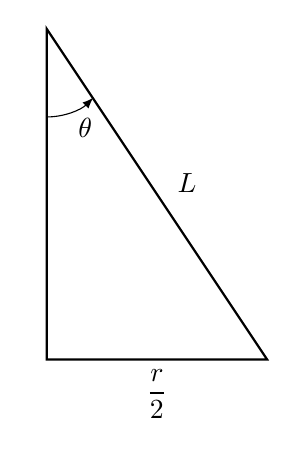
\begin{tikzpicture}[scale=1.4]

% Triangle
\draw[thick] (0,0) -- (0,3) -- (2,0) -- cycle;

% Labels
\node[left] at (0,1.5) {};
\node[right] at (1.1,1.6) {$L$};
\node[below] at (1,0) {$\dfrac{r}{2}$};

% Angle theta
\draw[->] (0,2.2) arc[start angle=270,end angle=315,radius=0.6];
\node at (0.35,2.1) {$\theta$};
\end{tikzpicture}
\end{center}

\noindent The sides are related through $\sin\theta$:
\begin{align*}
    \sin\theta = \frac{r/2}{L} \\
    \fbox{$\displaystyle\therefore r = 2L\sin\theta$}
\end{align*}

\noindent Express the forces in component form (Newton's 2nd Law) starting in the $y$-direction:
\begin{align*}
    F_{\text{net}} = 0 = T\cos\theta - mg \\
    \fbox{$\displaystyle\therefore T = \frac{mg}{\cos\theta}$}
\end{align*}

\noindent Similarly in the x-direction: 
\begin{align*}
    F_{\text{net}} = 0 = F_e - T\sin\theta
\end{align*}

Using the expression of $T$ in the y-direction, substitute into the $x$-direction equation: 
\begin{align*}
    F_e = T\sin\theta = \left(\frac{mg}{\cos\theta}\right) \cdot \sin\theta
\end{align*}
\end{tcolorbox}


\begin{tcolorbox}[
  colback=white,
  colframe=green!50!black,
  boxrule=0.8pt,
  arc=1.5mm
]

\noindent From Coulomb's Law: 
\begin{align*}
    F_e = \frac{k_e q_1 q_2}{r^2} \Rightarrow \frac{k_e q^2}{r^2} \Rightarrow \frac{k_e q^2}{\left(2L\sin\theta\right)} \\
    \therefore\frac{k_e q^2}{4L^2\sin^2\theta} = mg\frac{\sin\theta}{\cos\theta}
\end{align*}

\noindent Now put $\theta$ on one side of the expression: 
\begin{align*}
    \frac{\sin^3\theta}{\cos\theta} = \frac{k_e q^2}{4mgL^2}
\end{align*}

\noindent We could use a numerical approximation to solve LHS = RHS, but remember we have the small angle approximation:
\begin{align}
    \sin\theta \approx \theta \\
    \cos\theta \approx 1
\end{align}

Applying (6) and (7) into our expression:
\begin{align*}
    \frac{\theta^3}{1} &= \frac{k_e q^2}{4mgL^2} \\
    \vspace{0.5em}
    \Rightarrow \theta &= \left(\frac{k_e q^2}{4mgL^2}\right)^{1/3}
\end{align*}
\end{tcolorbox}

\subsection{The Vector Form of Coulomb's Law}
\label{sec:lecture4.1-vector-form}

\noindent Suppose we want the vector form of Coulomb's Law. We will use this illustration: 
\begin{center}
    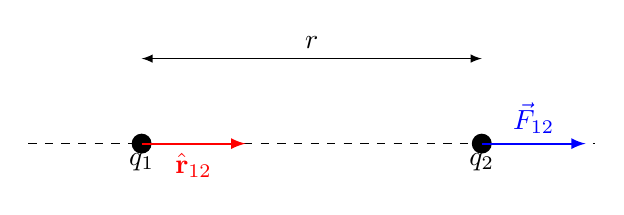
\begin{tikzpicture}[scale=1.2]

% Reference line
\draw[dashed] (-3,0) -- (3,0);

% Charges
\fill (-1.8,0) circle (3pt);
\node[below] at (-1.8,0) {$q_1$};

\fill (1.8,0) circle (3pt);
\node[below] at (1.8,0) {$q_2$};

% Separation r
\draw[<->] (-1.8,0.9) -- (1.8,0.9);
\node[above] at (0,0.9) {$r$};

% r-hat from q1 to q2
\draw[red,->,thick] (-1.8,0) -- (-0.7,0);
\node[red,below] at (-1.25,0) {$\hat{\mathbf r}_{12}$};

% Force on q2 due to q1
\draw[blue,->,thick] (1.8,0) -- (2.9,0);
\node[blue,above] at (2.35,0) {$\vec F_{12}$};

\end{tikzpicture}

\end{center}

\noindent We will define the unit vector $\displaystyle\hat{r}_{12}$:
\begin{itemize}
    \item vector of length 1 along the $x$-axis,
    \item $\displaystyle\hat{r}_{12}$ points from $q_1$ to $q_2$.
\end{itemize}

\noindent Consider the vector equation form:
\begin{align*}
    \vec{F}_{12} = \frac{k_e q_1 q_2}{r^2}\hat{r}_{12}
\end{align*}

\noindent If the product of $q_1$ and $q_2$ is positive (i.e. both positive or negative charges), then $\vec{F}_{12}$ points away from $q_1$, meaning it is repulsive. 

\vspace{0.5em}

\noindent If the product of $q_1$ and $q_2$ is negative (i.e. opposite charges), then $\vec{F}_{12}$ points towards $q_1$, meaning it is attractive.

\pagebreak

\section{The Electric Field}

\noindent The electric field is denoted by the symbol $\displaystyle\vec{E}$. Imagine a picture where a charge $\displaystyle q_1$ creates a $\displaystyle\vec{E}$-field in a space that exerts forces on other nearby charges. 

\begin{center}
    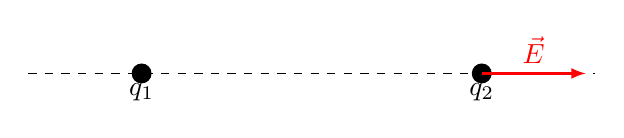
\begin{tikzpicture}[scale=1.2]

% Reference line
\draw[dashed] (-3,0) -- (3,0);

% Charges
\fill (-1.8,0) circle (3pt);
\node[below] at (-1.8,0) {$q_1$};

\fill (1.8,0) circle (3pt);
\node[below] at (1.8,0) {$q_2$};

\draw[red,->,thick] (1.8,0) -- (2.9,0);
\node[red,above] at (2.35,0) {$\vec{E}$};

\end{tikzpicture}

\end{center}

\noindent From this illustration, the force on $\displaystyle q_2$ due to $\displaystyle \vec{E}_1$ is:
{\large
\begin{align*}
    \displaystyle \vec{F}_{12} = q_2 \vec{E}_1
\end{align*}
}

\noindent The value $\displaystyle\vec{F}_{12}$ is known from Coulomb's Law, which precisely has a value of:
{\large
\begin{align*}
    \displaystyle \vec{F}_{12} = k_e \dfrac{q_1 q_2}{r^2} \hat{r}_{12}
\end{align*}
}

\noindent Therefore we require that: 
\begin{align*}
   \displaystyle q_2 \vec{E}_1 = k_e \dfrac{q_1 q_2}{r^2} \hat{r}_{12}
\end{align*}

$\displaystyle q_2$ cancels out: 
\begin{align*}
    \displaystyle \cancel{q_2} \vec{E}_1 = k_e \dfrac{q_1 \cancel{q_2}}{r^2} \hat{r}_{12}
\end{align*}

\noindent Therefore the $\vec{E}$-field due to point charge $\displaystyle q_1$ is: 
\begin{align}
    \displaystyle \vec{E}_1 = k_e \dfrac{q_1 }{r^2} \hat{r}_{12}
\end{align}
where $\displaystyle\hat{r}$ is a radial unit vector from the $\displaystyle q_1$ origin.

\subsection{Graphing electric field lines}
\noindent For a positive charge $\displaystyle q_1$, $\vec{E}$ points away from the charge. Usually these lines are drawn as continous lines: 
\begin{center}
    \includegraphics[scale = 1.5]{figures/efieldlinepos.pdf}
\end{center}

\noindent In this picture, the spacing between the field lines determines the strength of the field lines. 

\pagebreak

\noindent Since $\displaystyle \vec{E} = k_e \dfrac{q}{r^2}\hat{r}$, if $q < 0$, then $\displaystyle \vec{E}$ is anti-parallel to $\hat{r}$ which always points radially outwards. 

\end{document}
